
\documentclass[border={0pt 0pt 0pt 0pt}]{standalone}
\usepackage{tikz-cd,tikz-3dplot} 
\usetikzlibrary{calc,intersections,through,backgrounds,decorations.pathmorphing, decorations.shapes,decorations.markings,patterns}
%include other needed packages here   
\begin{document}
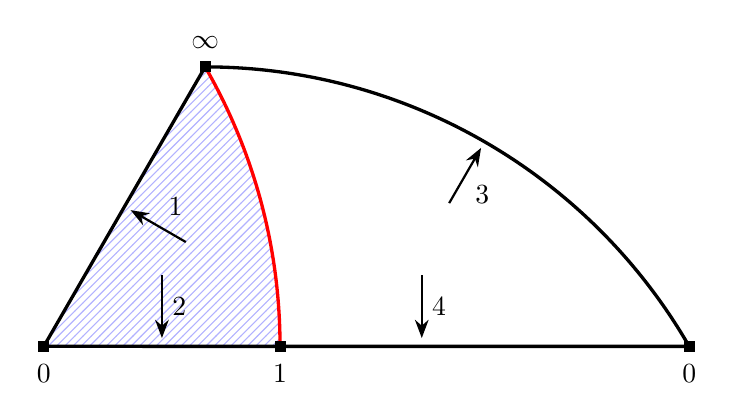
\begin{tikzpicture}[scale=3]
\def\a{2.366025403784439} 
\coordinate (A) at (0,0);
\coordinate (B) at (1,0);
\fill[pattern=north east lines, pattern color=blue!30!white](A) -- (B) arc [start angle=0, end angle=30, radius=\a] coordinate(C)  --cycle;
\draw[very thick] (A) -- (C) node [midway](E) {} arc [start angle=-90, end angle=-150, radius=-\a] coordinate(D) node [midway](F) {} --cycle;
\draw[very thick,red] (B) arc [start angle=0, end angle=30, radius=\a];

\foreach \point/\position/\lab in {A/below/0,B/below/1,C/above/\infty,D/below/0}
{
	\node [fill=black,inner sep=2pt]  at (\point){};
	\node[\position=3pt] at (\point) {$\lab$};
}
\foreach \y/\ytext in {0.5/2,1.6/4}
\draw[-{Stealth[]},thick] (\y cm,0.3cm) to node[anchor=west] {$\ytext$} (\y cm,1pt);
\foreach \y/\ytext/\angl/\place in {E/1/-30/south west, F/3/-120/north west}
\draw[-{Stealth[]},thick] ($ (\y) + 0.3*(cos \angl, sin \angl) $) to node[anchor=\place] {$\ytext$} ($ (\y) + 0.03*(cos \angl, sin \angl) $);
\end{tikzpicture}
\end{document}